\subsection{Paramètres du solveur temporel}
\begin{table}[H]
\centering
\begin{tabular}{lcc}
\toprule
Paramètre & Symbole/mot-clé & Valeur \\
\midrule
Pas de temps minimal & $\mathrm{d}t_{\mathrm{min}}$ & $10^{-3}$~s \\
Pas de temps maximal & $\mathrm{d}t_{\mathrm{max}}$ & $10^{3}$~s \\
Facteur de sécurité & \texttt{facsec} & $10^{7}$ -- $10^{8}$ \\
Facteur de sécurité maximal & \texttt{facsec\_max} & $10^{8}$ -- $10^{9}$ \\
Seuil de convergence (solveur linéaire) & -- & $10^{-1}$ \\
Seuil de convergence (schéma implicite) & -- & $10^{-1}$ \\
Seuil de stationnarité & \texttt{seuil\_statio} & $10^{-5}$ \\
\bottomrule
\end{tabular}
\caption{Paramètres du schéma temporel implicite utilisé pour la convergence vers l'état stationnaire.}
\label{tab:solveur}
\end{table}



\subsection{Résultats détaillés du cas à $980$~K} 

Cette partie détaille les résultats de sensibilité à la discrétisation axiale $N_z$ pour le deuxième niveau de puissance étudié dans ce rapport ($4~\mathrm{MW/m^3}$, température moyenne d'assemblage $\overline{T}\approx981{,}4$~K), en complément de la synthèse présentée au corps du rapport (Section~\ref{sec:consequence_radiosite}).

La Figure~\ref{fig:temperature4MW} compare les champs de température obtenus avec $N_z=4$ et $N_z=20$, ainsi que leur différence. La Figure~\ref{fig:convergence4MW} présente l'évolution des écarts relatifs des températures minimale, maximale et moyenne en fonction de $N_z$, par rapport à la solution de référence.

\begin{figure}[H]
\centering
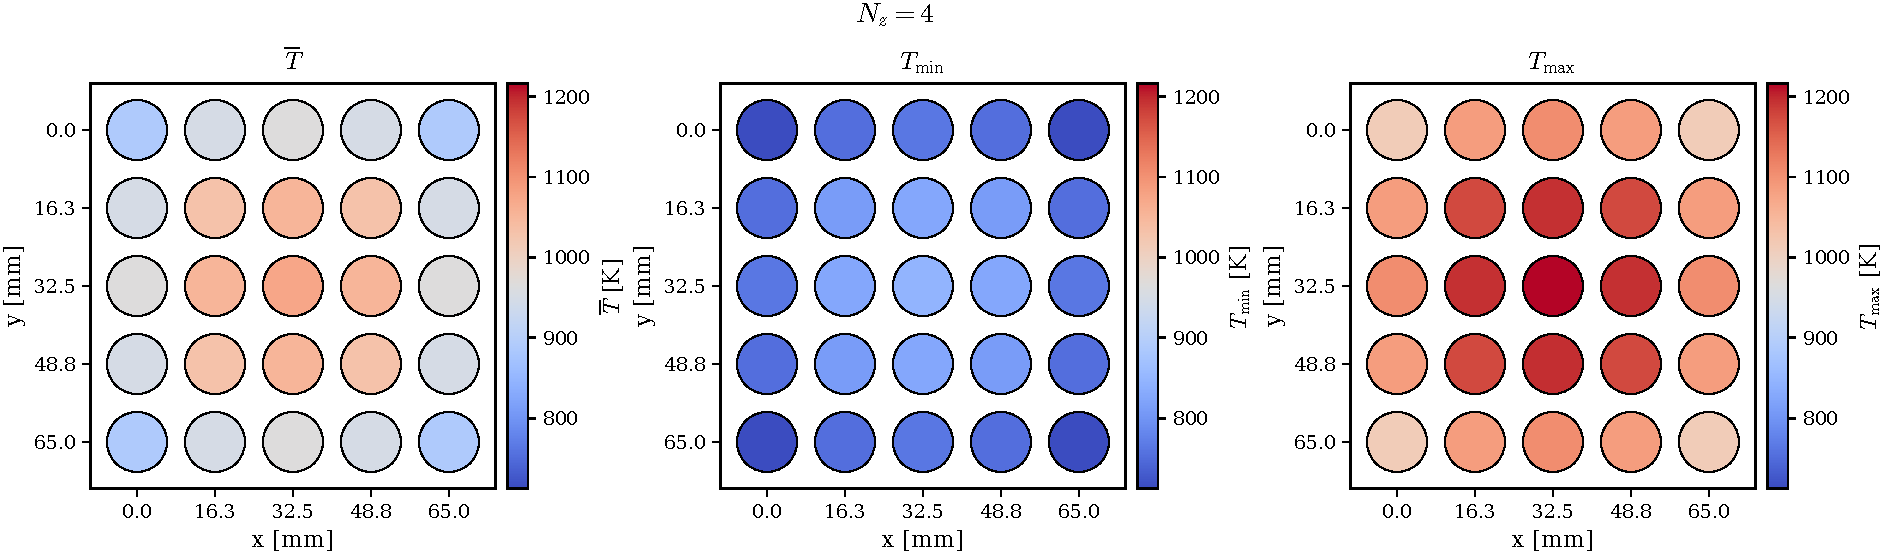
\includegraphics[width=0.8\linewidth]{PICTURES/c5couplage/T1000/assembly_4.pdf}

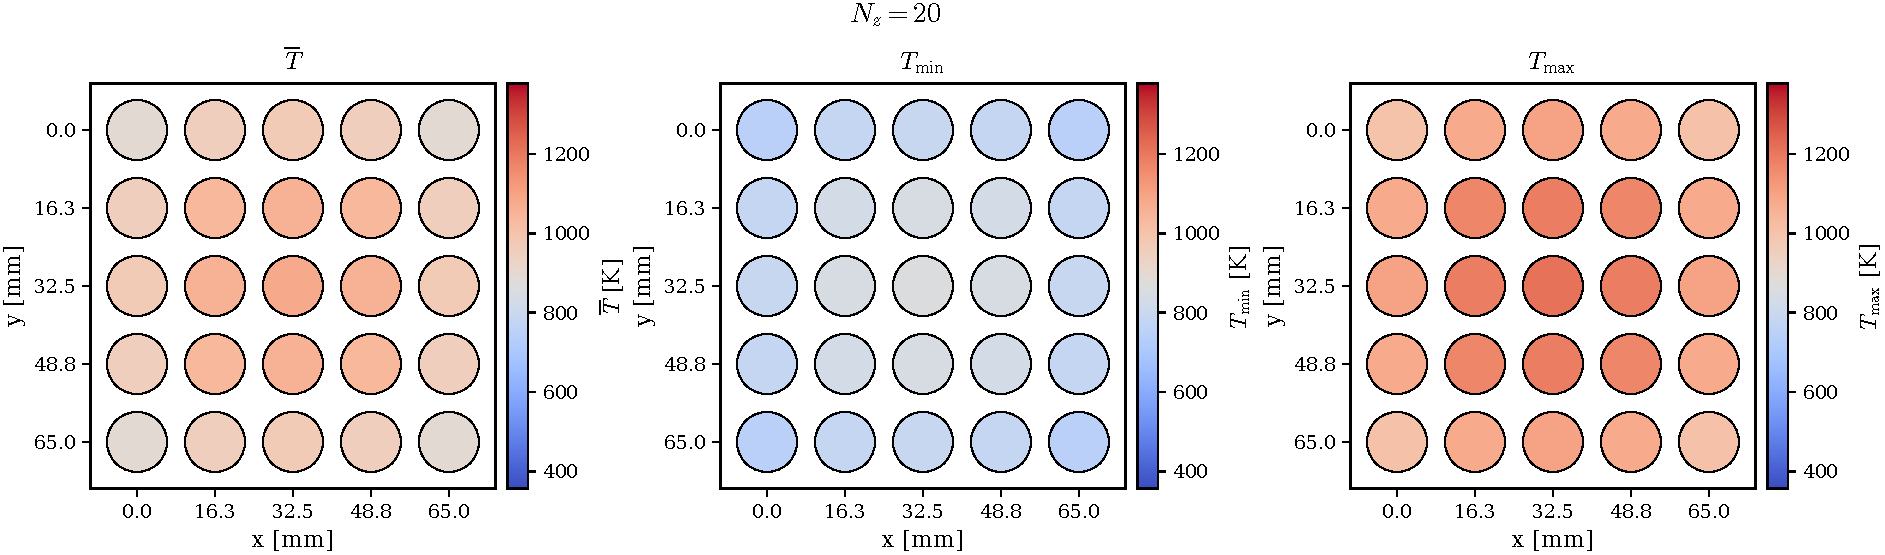
\includegraphics[width=0.8\linewidth]{PICTURES/c5couplage/T1000/assembly_20.pdf}

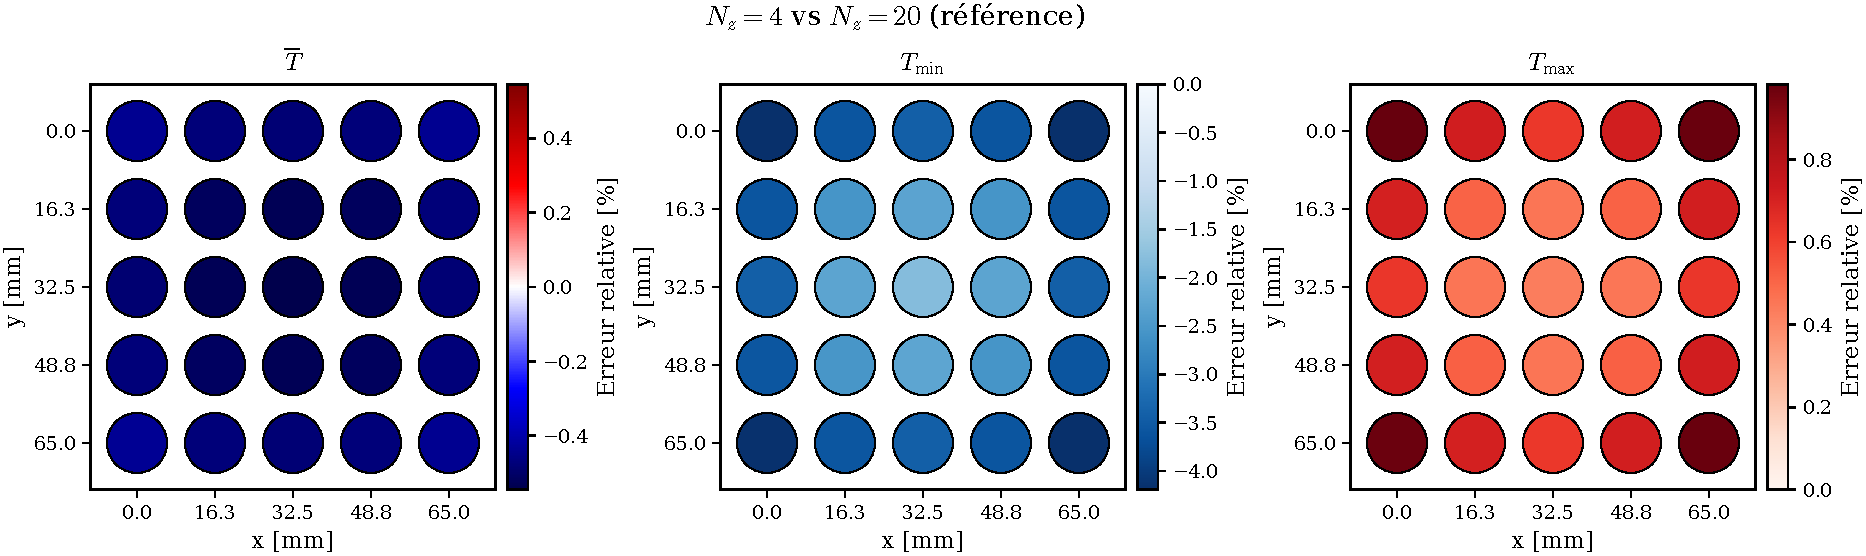
\includegraphics[width=0.8\linewidth]{PICTURES/c5couplage/T1000/assembly_diff_4_vs_20.pdf}
\caption{Champs de température pour $\overline{T}=981{,}4~\mathrm{K}$ : $N_z=4$ (haut), $N_z=20$ (milieu) et différence entre les deux champs (bas).}
\label{fig:temperature4MW}
\end{figure}

\begin{figure}[H]
\centering
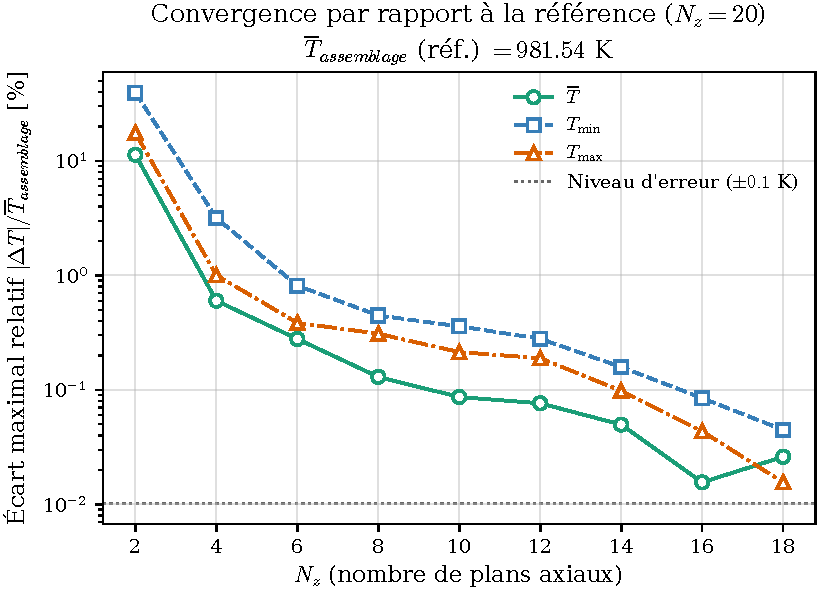
\includegraphics[width=0.7\linewidth]{PICTURES/c5couplage/T1000/convergence_relative_vs_20.pdf}
\caption{Écart relatif des températures minimale, maximale et moyenne en fonction de $N_z$, par rapport à la référence $N_z=20$, pour $\overline{T}=981{,}4~\mathrm{K}$.}
\label{fig:convergence4MW}
\end{figure}

Comme pour le premier niveau de puissance, on observe une convergence vers la solution de référence, sans modification de la structure thermique globale de l'assemblage : le crayon central demeure le plus chaud, les crayons d'angle les plus froids, et la discrétisation axiale ne modifie que les niveaux locaux de température.

La hiérarchie des écarts observée précédemment est également conservée, mais leur amplitude augmente légèrement : $T_{\max}$ est surestimée jusqu'à $0{,}9\,\%$ (contre $0{,}7\,\%$ pour le niveau de puissance précédent), tandis que $T_{\min}$ et $\overline{T}$ sont sous-estimées jusqu'à $4\,\%$ et $0{,}5\,\%$ respectivement (Tableau~\ref{tab:ecarts_discretisation_axiale_4MW}).

\begin{table}[H]
\centering
\caption{Écarts relatifs maximaux observés par rapport à la référence $N_z=20$ pour $\overline{T}=981{,}4~\mathrm{K}$.}
\label{tab:ecarts_discretisation_axiale_4MW}
\begin{tabular}{lcc}
\hline
Grandeur & Sens de l'écart & Écart maximal \\
\hline
$T_{\max}$ & Surestimation & $+0{,}9\,\%$ \\
$T_{\min}$ & Sous-estimation & $-4{,}0\,\%$ \\
$\overline{T}$ & Sous-estimation & $-0{,}5\,\%$ \\
\hline
\end{tabular}
\end{table}

Cette légère amplification, par rapport au cas de puissance précédent, est cohérente avec la physique du transfert radiatif discutée en Section~\ref{sec:consequence_radiosite} : la dépendance en $T^4$ de la loi de Stefan--Boltzmann confère au flux radiatif une sensibilité relative quatre fois supérieure à celle de la température elle-même, de sorte qu'à erreur relative de représentation constante, l'erreur sur le bilan radiatif croît avec le niveau de température. L'augmentation de la puissance accentue par ailleurs les gradients thermiques, élargissant l'écart de l'inégalité de Jensen et dégradant d'autant la représentativité d'une température homogénéisée. Comme dans le cas précédent, l'erreur se concentre sur les températures extrêmes, la température moyenne bénéficiant de compensations spatiales.

La vérification de la convergence du solveur confirme, comme pour le cas précédent, que les écarts observés ne proviennent pas d'une insuffisance de convergence numérique : avec une température moyenne stabilisée à $0{,}1~\mathrm{K}$ près, l'incertitude relative associée est de l'ordre de

\begin{equation}
\frac{0{,}1}{981{,}4}
\approx 1{,}0\times10^{-4},
\end{equation}

soit au moins un ordre de grandeur en dessous des écarts mesurés, qui atteignent plusieurs pourcents sur $T_{\min}$. Les écarts observés sont donc bien imputables à la discrétisation axiale.

Ce deuxième niveau de puissance confirme ainsi les conclusions établies pour le premier cas : la solution converge vers un état indépendant de $N_z$ lorsque la discrétisation s'affine, la structure thermique globale est préservée, et l'erreur de représentation radiative s'amplifie modérément avec le niveau de température, conformément à la sensibilité en $T^4$ des échanges radiatifs.
